\section{Problems}
There are a lot of problems regarding how we treat the problem, how we see it, and how we actively analyze it. Most of them lies in the space of statistical learning theory, since bias-variance on itself has variations and justification that is seemingly very natural in statistical theory, like the other version name \textit{approximation-estimation error tradeoff}. All of them contribute somewhat to the current outlook, and so far, it has been pretty bad, than what is being advocated of. Nevertheless, let us state them out, even if missing some particular details. 

\subsubsection*{Problem 1. Authoritative statements}
Despite its prevalence in particular research interest, double descent itself has no definite statement to describe its particular behaviour. This is also true for a list of other phenomena, such as \textit{grokking} (\cite{power2022grokkinggeneralizationoverfittingsmall}), \textit{emergence behaviours} (\cite{wei2022emergentabilitieslargelanguage}, typically discussed in large language models, which is understandable of large-scale specific ruling system), \textit{implicit bias} (\cite{soudry2024implicitbiasgradientdescent}), and \textit{neural scaling law} (\cite{kaplan2020scalinglawsneurallanguage,wei2022emergentabilitieslargelanguage}). There is also \textit{catastrophic forgetting} (\cite{vandeven2024continuallearningcatastrophicforgetting}) which is still fairly native of large systems; nevertheless, those phenomena will be of target later on (or discussed in later chapters). The fact remains that we only \textit{partially understand} these particular results with conjectures and theories to support the facilitation of new insights, new analytical lens, and nothing much. Without a clear definition of what is even double descent, sometimes, we cannot proceed, lest to say even solving it. This is a problematic issue, since the current theory is so messy and not rigid that many even turns to exotic choices, like topological informatics learning theory, \textit{Homotopy Theoretic and Categorical Models} (\cite{Manin_2024}), and several more. Without clear definitions, it remains ambiguous whether double descent constitutes a single phenomenon, a family of related behaviours, or an artefact of particular modelling and evaluation choices. 

More fundamentally, the term \textbf{double descent} does not currently admit a formal definition beyond an empirical characterization of observed risk behaviour. While several works have suggested interpreting double descent as an instance of emergent behaviour, such interpretations necessarily remain conjectural, as emergence itself lacks a precise and operational definition within contemporary learning theory. As a result, appeals to emergence do not resolve the underlying indeterminacy of the phenomenon, but rather shift it to a different conceptual level.

Empirically, double descent has been reported in a variety of settings, while being absent in many others, even under closely related modelling and data conditions. This variability complicates attempts to treat double descent as a unified phenomenon and raises the question whether it constitutes a single mechanism, a collection of regime-dependent effects, or an artefact of specific modelling and evaluation choices. In the absence of necessary and sufficient conditions for its occurrence, theoretical accounts are forced to accommodate mutually incompatible behaviours, thereby undermining their explanatory specificity. Consequently, existing frameworks face a dual difficulty: they neither reconcile naturally with classical bias-variance analyses, nor align with the assumptions underlying earlier generalization results, such as uniform convergence over well-behaved hypothesis classes. Without a precise characterization of the object under study, it remains unclear how such theories can be systematically compared, falsified, or extended.

\subsubsection*{Problem 2. Model complexity}
The notion of model complexity has undergone a significant conceptual shift in the recent literature. Several works have attempted to formalise or reinterpret model complexity in modern learning systems \cite{hu2021modelcomplexitydeeplearning,luo2024investigatingimpactmodelcomplexity,barcelo2020modelinterpretabilitylenscomputational,Molnar_2020,janik2021complexitydeepneuralnetworks}. This problem becomes apparent when the inherently complex nature of contemporary models—particularly deep learning models based on multilayer perceptron (MLP) architectures—is examined, as such models cannot be treated analogously to classical hypothesis classes.

In \cite{hu2021modelcomplexitydeeplearning}, deep learning models are analysed through notions such as expressive capacity, effective capacity, VC dimension, and proxy-based Rademacher complexity bounds, alongside perspectives grounded in functional analysis, computational complexity, and representational width. However, these approaches remain largely heterogeneous and regime-dependent. Notably, \cite{Molnar_2020} demonstrates the possibility of decomposing model behaviour into multiple contributing notions of complexity, suggesting a unification at the level of functional variation rather than a single scalar measure.

Despite these advances, there remains no conclusive or universally accepted definition of model complexity. This ambiguity becomes particularly problematic in light of phenomena such as double descent, which have been observed not only in deep learning models but also, inconsistently, in classical settings \cite{belkin_reconciling_2019}. As a result, the issue is foundational: theoretical analysis of generalisation behaviour presupposes a well-defined notion of complexity, especially when complexity itself is the variable of interest.

Relatedly, the concepts of overparameterization and underparameterization lack precise and agreed-upon definitions. Their usage is often context-dependent and implicit, yet they play a central role in the classification of problem settings and the interpretation of learning dynamics. Without explicit characterisation of these notions, theoretical comparisons across models and regimes remain inherently ambiguous. Absent such definitions, claims relating model complexity to generalisation behaviour risk being descriptive rather than explanatory.

\subsubsection*{Problem 3. Model structure}

In modern practice, the theoretical and formal treatment, rigorous consideration of different model structures and complexity is not realized. Partially, this is due to the bloom of machine learning and artificial intelligence from the early 2000s. Currently, there has been no conclusive theoretical definition or formulation about the structure of different models, typically can go under the name of mathematical modelling hypothesis, in a way that unify certain properties between architectures. Heuristics are also often employed in several newer models and widely-utilized structures typically seen in large-scale systems, leading to difficulty in formalization and factorization of affectants. 

\subsubsection*{Problem 4. Theoretical insufficiency}

The setting surrounding the learning theory, machine learning models is generally missing of its rigours and analytical properties. Most of the learning setting and model's training-testing setting are often narrowly stated in theoretical sense, and there are a lot of diffusing details that might or might not affect the model's perturbation without knowing. This in a certain way leads to the complexity in analysing different problem setting and experimental results, since the architecture used, the setting considered, model in questions, configuration (either custom or on system side) are not consistent overall. 

Furthermore, a lot of terms, definitions are often hand-waived in papers or in discussions. This also led to the point that in \cite{nakkiran_deep_2019}, they have to somehow 'reinvent' another type of model complexity itself, albeit unsatisfying of a definition, is still a new kind of definition per insufficiently of such. while it is welcome to introduce new definitions, the fact is that it is subjectively inconclusive of terms, definitions and thereof leads to the perception and situation where multiple studies can be found, but all of them are defined on different ground.

Analysing statistical learning theory and overall landscape of statistical learning theory, and the learning theory as a whole, encountering new problems like double descent also revealed its weakness, and ultimately, perhaps one of the reason why it is ineffective against such problem. First, there are simply too many assumptions made, too many formulations made during said process. Furthermore, there are also unclear notions and concepts, of which make it even harder to analyse or fully formalize. Secondly, there are inherent conflicts and uncertainty within those theories, formulations and notions by itself. For example, in one sense, the No-free-lunch theorem is considered to be representative and true, whilst also simultaneously being considered the opposite of such. And amidst abnormality behaviours of the old bias-variance formulation, we also find distinctive weakness in our theory, for example, the concerning difficulty in defining the notion of \textit{model complexity} in various contextual ways. To analyse double descent, perhaps we also need a new theory or formulation to support it. \footnote{Furthermore, most of the general solution and bounds created by statistical learning theory is often in a very simplistic system. For example, if we are to utilize the Rademacher complexity measure (\cite{10.5555/2371238}), most of the time we will have to compute it through the growth function $\Pi_{\mathcal{H}}(m)$ for $m$ points, on the standard finite hypothesis class $\mathcal{H}$ such that 
\begin{equation}
    \Pi_{\mathcal{H}}(m) = \max_{x_1, \dots, x_m \in \mathcal{X}} \left| \left\{ (h(x_1), \dots, h(x_m)) \mid h \in \mathcal{H} \right\} \right|
\end{equation}
Most of our problems resolve to binary classification, or rather, the problem of pattern recognizing discrete, reduced classification form. It is not so sure for now if all problems can be reduced to such way, so we cannot draw conclusive analysis that is not diluted of mathematical formulation for complex systems. That is not to count the computationally intensive operation required to calculate the supposedly classical measure, while not entirely of itself holds any substantial reasonable information about the internal dynamics of the model itself. }

Another problem with classical analytical solution is that it is very \textit{loose}, almost too loose to even considered of such. But sometimes it is too \textit{rigid} in a sense such that it simply does not work at all. Indeed, basing our works and foundational assumptions on top of approximation theory is not quite good at all, because they are very limited. Overall, we can say it is not equipped for handling similar situation. For example, almost all bounds that is subjected of classical learning theory only guarantee particular existential theorem, under very simplified and specific situation without the virtue of extending it to a more general setting. 


%%%%%%%%%%%%%%%%%%%%%%%%%%%

\section{Principle}

We are motivated from earlier analysis, further experimental results, and arguably practical observations of empirical-based architectures that we find interesting. Oddly enough, the idea is encouraged of the observation that \textit{deep neural network} organising architecture might be more general than it is, particularly in the sense of mathematical modelling and structural implicit approximation, as well as factors like scalability, generality, and else. Furthermore, one of the purpose of this novel theory is also to redefine the entire learning space to, at least if not entirely original, might as well fall into the category of a reformulation of theoretical framework and not partaking the role of replacing it. 

As such, we need some principles to get started the analysis. What can those be that guarantee the success of a particular reformulation at first? For starter, we indict on the requirement of developing a general framework of neural network-like organisation for our models, both in the interpretation of the learning objective, and the structure of the hypothesis learner. Secondly, we have to define learning as a barebone process, of which then we will have to justify \textit{probabilistic nature} of it and the degree in which that is true. Thereby, we will then also have to reconsider the learning problem, under what scope of the problem and the classes of learning that is there to be achieved, the encoding space and what it is meant to, and the criteria of guaranteeing such learning to be probable. For now, those are enough, but the development that come afterward will justify it instead of the principle. 

Indeed, we can see the principle here - we want to redefine learning process in an organized manner, with minimal messiness from considering all factors together, and normalize the interpretation of \textit{unit-wise} architecture that neural network uses up to more. 

\subsection{Structures}

Then, what is the plan? The goal is to \textit{systematically introduce} the concept and the novel theory. Hence, we will separate it into discrete small step size parts. First, we need to conform the setting with a new template. This mean the following order is needed. 
\begin{enumerate}[leftmargin=1cm,itemsep=2pt,topsep=2pt]
  \item Introduce and define the formalism of an \textit{ambiance space} and an \textit{encoding space}. Those two will come in together to form the majority of $S$ as per system dynamic notation. 
  \item In the \textit{collection} $S$ should we extend it further, there always exists the object $h$, belonging to certain configuration class $\mathcal{H}$. We need to define this particular object, and its interaction to the collection itself. Which means, the ambiance space and encoding space. How do we bring up the \textit{representation concept} here altogether? 
  \item To start the mechanics, we need the \textit{mechanical space} $M$ to be defined. What can be it? What connects and form the structural description that $S$ make with the ambiance space, encoding, representation, subject dynamics, and else? 
  \item Now, come to the \textit{operational process}. For this, let's assume we have two different systems, in accordances, $S_{1}$ and $S_{2}$, each of which houses $h$, and $c$ respectively. How do they communicate? How, should it be done, can the operational space indict particular objective, or requirement, such that $h$ is evaluated, and $c$ is evaluated? What is hidden of $h$, and what is hidden of $c$? 
  \item Then, finally, bounds, theorems, analytical results, algorithmic consideration and conjectures that fit, into this description. 
\end{enumerate}
From the scope of it, it might seem not too practical to call as novel. But as far as we are considered, there should be something to take account on, and we need to do them carefully, such is to say there has been none, of which partake in said direction. There is a reason why messy construction being the worst nightmare of any people using the house, and we are the one to fix it, or at least attempted so. 

\section{Precursor}

We begin by the analysis on the concept of \textbf{system space}. Fundamentally, the purpose of system space is to specify everything that contributes to the system dynamic. Or rather, any component, objects, subject structures, and so forth that acts, that exist, that is considered of interest in a given context. The principle is simple, to separate between the \textit{assumed shape} of an object from it representation or encoding. This can be done by specifying two parts - the \textit{ambiance space}, of which contains all the object in consideration, minus their properties and so of, and the \textit{encoding space}, which as its name implies, encodes all relevant structural information and properties that is considered, of said object. Just consider the very simple example of a car, specifying the barebone existence of it in an operational space, and the encoding space of the specific details of such cars, and factors affecting such. 

Before doing anything, let us define what is meant by ambiance space, and subsequently, encoding space, via a more statement-form definition. First, let us define the \textit{system space}. 
\begin{definition}[System space, Preliminary version]
  For any `procedural' structures, objects, realization \footnote{In the sense of explicit construction like coding, creating models that will have to be evaluated, instead of mathematical static statements and of operational means.}, we define the \textit{system space} $\mathcal{S}$ as the space containing two types of facilities that support it, the \textit{ambiance space} for where objects are realized, and the \textit{encoding space} where their realization is encoded and supported of its operation. 
\end{definition}

Hence, in essence, the system space includes, and contain the realization of the object itself. Such object can be anything, apple, baskets, logical system, interpretable text structure, 'unstructured data' in a sense, and so on. The accompanying space of the system space, however, is the encoding space. 

\begin{definition}[Encoding space, Preliminary version]
    The encoding space $\mathcal{E}$ of particular system space $\mathcal{S}$, contains the information and structural encoding of objects of the ambiance space $\mathcal{A}$, within certain representation scheme. 
\end{definition}

The ambiance space is simply defined as followed, of which contains the ambiance of the system. 

\begin{definition}[Ambiance space, Preliminary version]
    The ambiance space $\mathcal{A}$ is defined as the collection of objects of interest, with minimal observational language specifying it, and contain the raw, non-encoded subject of interest. 
\end{definition}

This contrast, even though we take inspiration from it, the ambiance space in the context of mathematical geometry and the like. For mathematics, the \textit{ambiance space} of a given object $x$ is the surrounding space of that mathematical object. So, if we study $\{x\}$, then its ambiance space is the $\mathbb{R}$ set. If $x$ is specified to be of high-dimension, then so on for $\mathbb{R}^n$. 

\begin{figure}[htb]
  \centering
  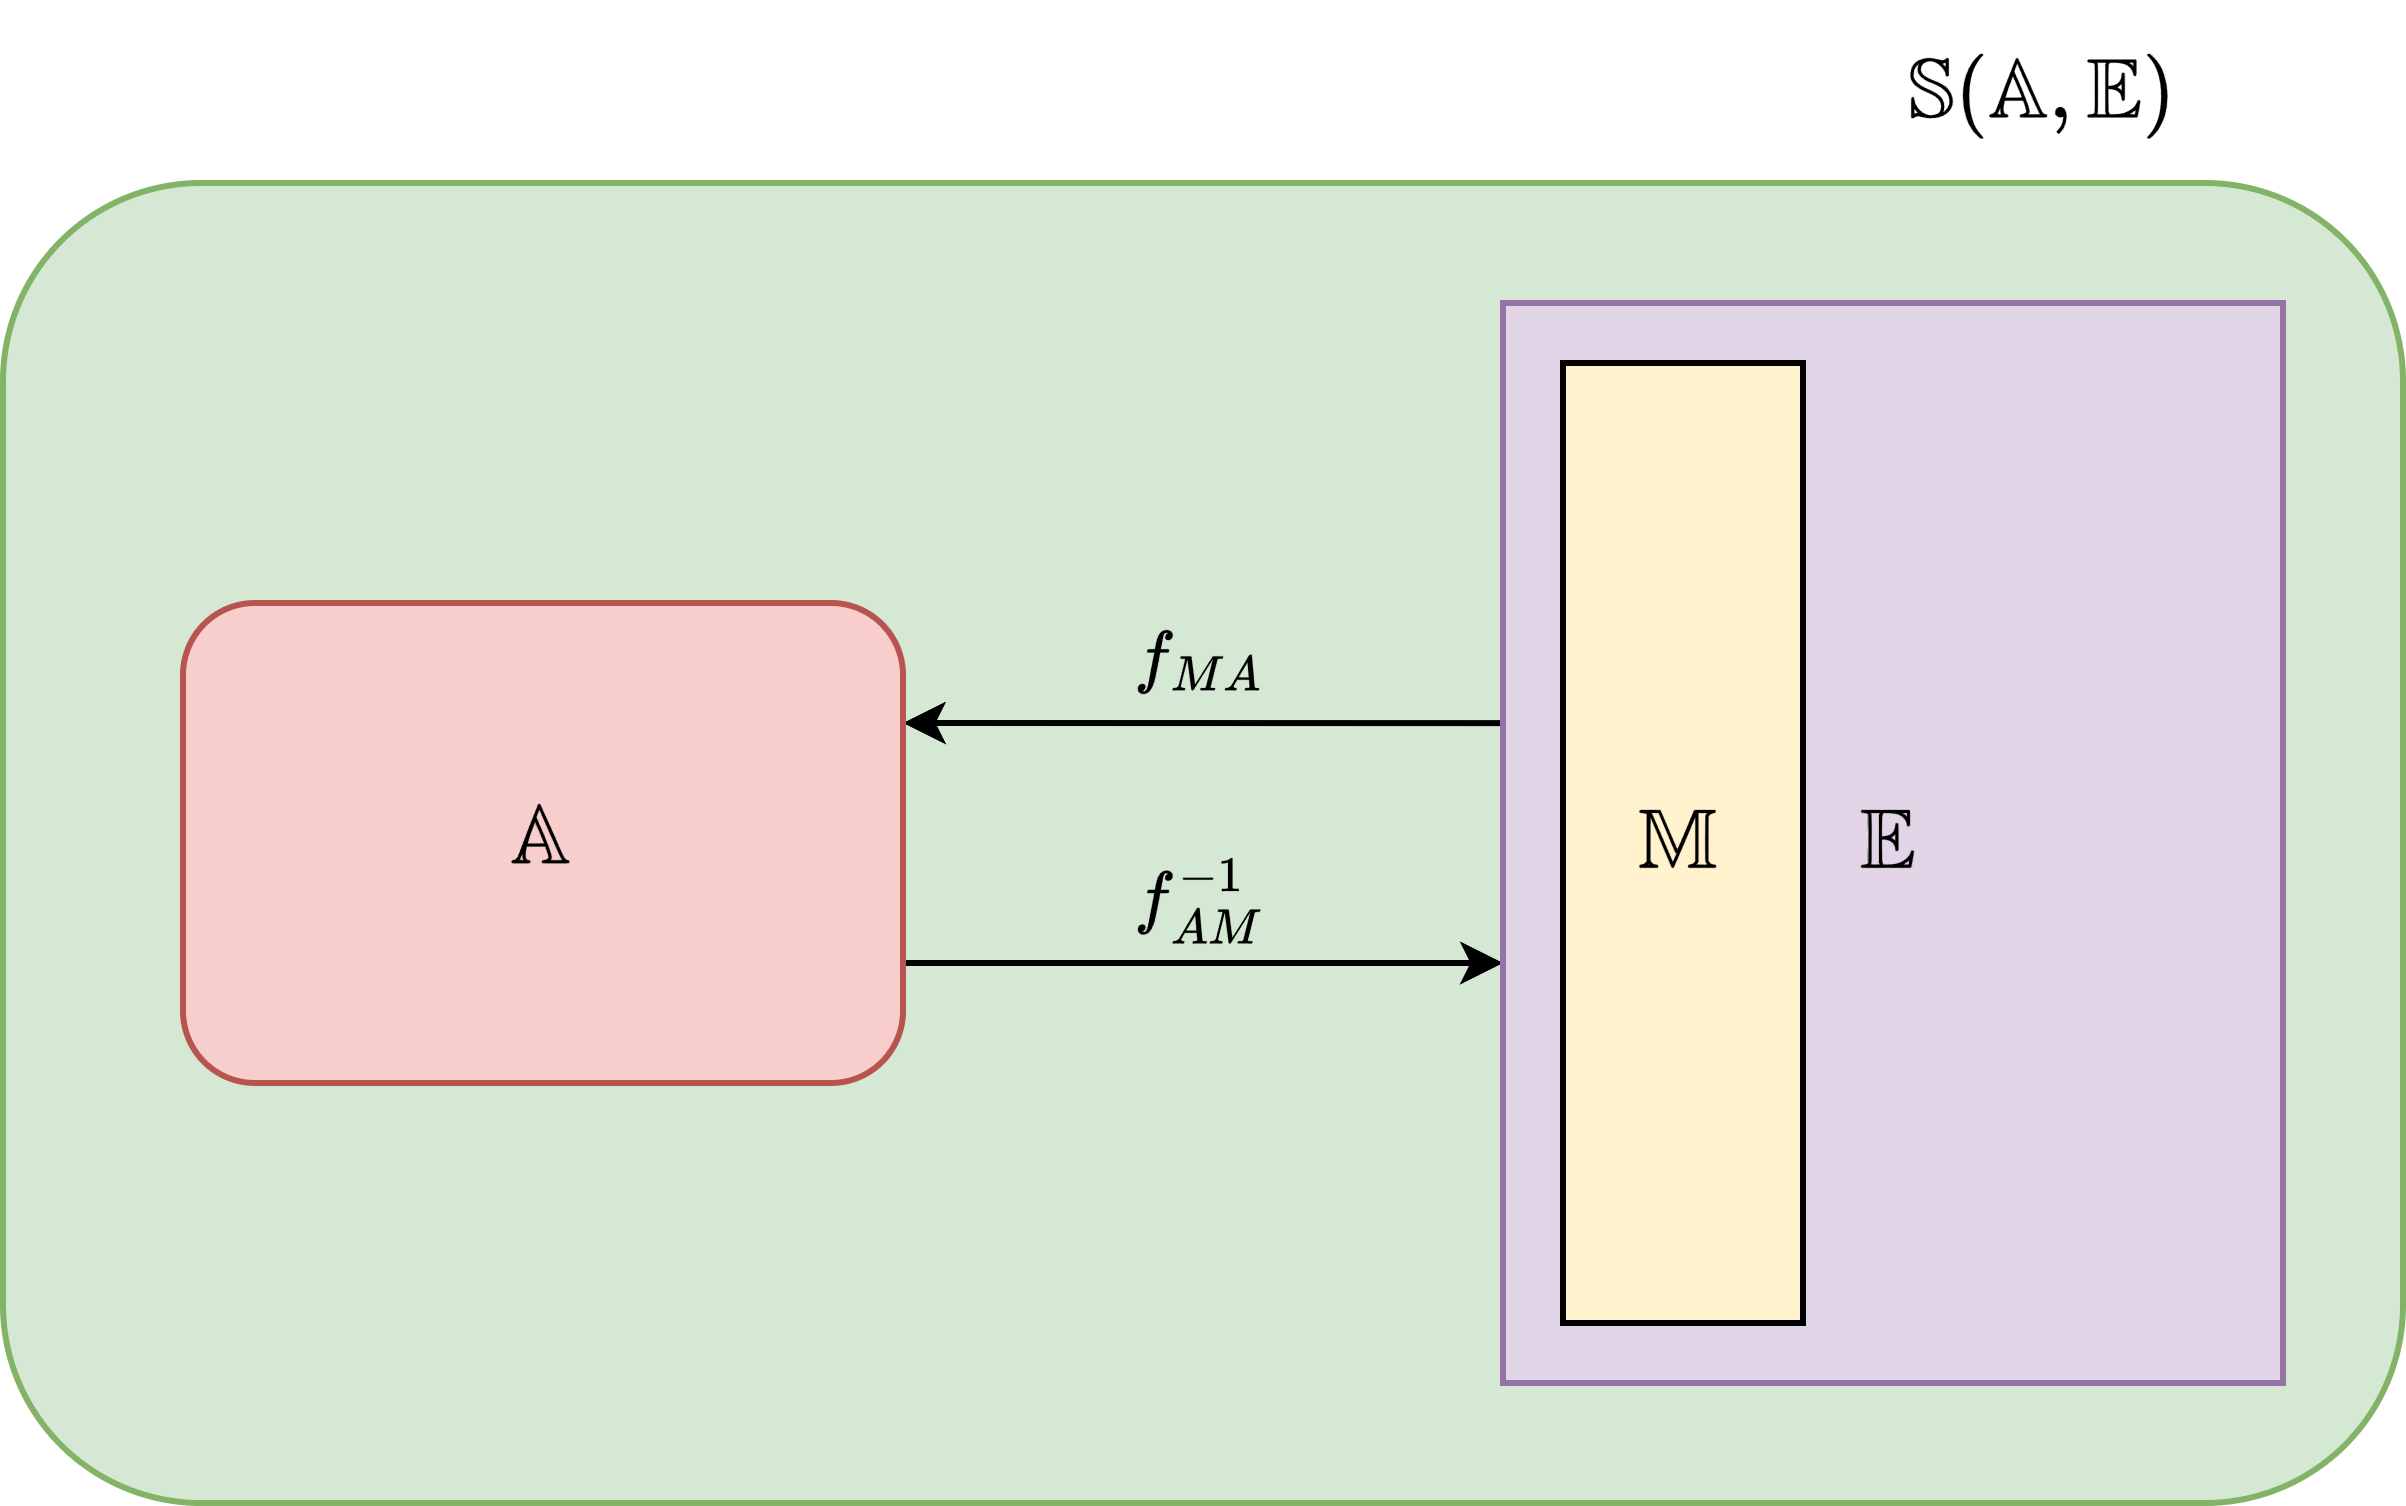
\includegraphics[width=0.5\textwidth]{img/model_representation.png}
  \caption{\textbf{Illustration of ambiance and encoding space, alongside a specific structural compact on the encoding}. The notation shifted to $\mathbb{A,M,E}$, but nevertheless represents the same structure. Here, as we can see, the system space contains ambiance and encoding space, alongside a specific encoding-related structure $\mathcal{M}$, and then two decoding and encoding which is short for interpreting between the two encoding spaces.}
\end{figure}

We understand this as inference of structures and objects into an interpretable and operational form. Specifying structures of certain objects, specifying properties of certain objects, the process of describing starting from static form, is inferred in the encoding sense. To encode objects, then in the ambiance space, require a representation framework that is powerful or rigid enough, to express particular properties and descriptions available to describe such object. We call it also the \textit{language} $\mathcal{L}_{E}$ of the encoding space, and subsequently, of the system space. 

The definition of the ambiance space is fairly arbitrary. What can be made of it to specify $\mathcal{A}$ more concretely? The space of objects has its own minimal language, we denote as $\mathcal{L}_{E}^{*}$. Taking inspiration from quantum physics, the ambiance space captures the \textit{state} of the system to a given particular \textit{state space}, the cardinality or size of the system in consideration, and object's structure of state space level. To clarify this, we can look both of the encoding of abstraction. An object $x$ has two type of general description - the overall $x$ state, lies in the state space $\mathcal{X}_{S}$, and the specific $x$-only description, the description space $\mathcal{X}_{D}$. These two spaces work alongside each other. For example, in the static case, $x$ has no variation, the state space and the description space is related such that there will be a description for specific state of $x$ in $\mathcal{X}_{S}$, and vice versa of a corresponding state. For a dynamic system, then, of any variation from $x_{1}\to x_{2}$ in the state space, then there exists a quantified variation that explains such variation in the state space. Conversely, if one wish to vary certain description of the description space, then there will have to exist a corresponding variation in the state space. This is a simple concept, but explains the relation between them. Coincidentally, the state space is described, within and of the ambiance space, and encoding space for the description space. 

Given the system $\mathcal{S}=(\mathcal{A},\mathcal{E}(\mathcal{L}_{E}))$ by then, There exists the encoding function, $f_{e}: \mathcal{A}\to \mathcal{E}(\mathcal{L}_{E})$ by functional notation. There also then exists the inverse mapping $f_{e}^{-1}$. These are called \textit{correspondence functions}, and we should know how to express them in later section of interest, when we start working on the construction of the learning theory on top. For now, though, the main function of them is to relate between the two spaces together, as 

\subsection{Groundwork of systems}

The system itself has some particular structures and working relations altogether, such as given by the definitions above. As we explained, the system itself contains two spaces copulated together. Let us examine it with an example. 

Let take a system $\mathcal{S}_{0}$. This system contains the ambiance space of response paradigm, for example, if in physics, the set of particles observations in specific potential landscape - for example, inside a potential well or not. Then, we have the ambiance space $\mathcal{A}=\{a_{i}\}^{n}$ of such particles. The minimal language here is the positional intrinsic space $(x,y,z,\dots)$. The reason why in this case we choose it is because it is intrinsic of the object by itself - the object exists in such space, instead of the object draws out such description by itself. The encoding space then, includes the language $\mathcal{L}_{E}$, with alphabet or description sets $\{p_{1},p_{2},\dots,\}$. In our case, then, the role of the language is to describe the object via the encoding space, and certain relation of it. 

A property $p_{i}\in \mathcal{E}$ is \textit{connected} (dependent) to the ambiance space $\mathcal{A}$, if for all taken expression of $p_{i}$ for any corresponding $x_{i}$, then $p_{i}$ is per definition, not of a constant quantity. If it is, then $p_{i}$ is unconnected (independent) of the system description. Such is for example, the mass $m$ of the particle at any given point is a static and constant quantity, but electric charge $q$ or something else, might depend on the configuration in the ambiance space for its quantification to take effect. Certain quantity depends on the evolution of $x_{i}$ over specified axis, usually time $t$, to be specified, for example, velocity, or displacement. Such are secondary quantity, and is harder to define. 

We can also remove and strip down everything to its most natural state in the ambiance space. That is, to make the object to be totally abstract as a singular existential state. It is similar to asking an apple to exist, with the only description now available is the cardinality of the object itself. And in such sense, we can then also use a fairly typical view of \textit{graph theory} to aid in such description. However, as said, we must be very careful when introducing new concepts of interpretations. 

These two languages, $\mathcal{L}^{*}$ and $\mathcal{L}_{E}$ are what called the \textit{configuration} of the system. Without it, the system itself cannot exist, because they form the basis of forming the model and the system the model lives and acts on. How can we relate them? For once, as we argued of the state space, the state of the system at large can be considered, strip to bare minimum, an \textit{object cardinality language}. 

\begin{definition}[Ambiance language]
  The language $\mathcal{L}^{*}$ of the ambiance space $\mathcal{A}$ of arbitrary size and shape, can be expressed minimally into the \textit{object cardinality class} (OCC) in which every object is specified by the pair $(i,y)$ for identifier $i$ and cardinality $y$. Hence, in general, the minimal OCC is the space $(I,\mathbb{N})$, for arbitrary identifier.
\end{definition}

At this point, an inquiry must be pointed at. The use of the word language in our formal treatment is not similar to the usual language typically seen in of mathematics and the like. It can be, or should be, referred to as the operational or representation language instead. Mathematically speaking, we can consider it a wrapper on the standard mathematical language. Thereby, a lot of components we use would be taken without proof or formalism required, out from the mathematical language itself. So what is it that we are actually using? These languages have the role to describe the system in certain manner only, within a scheme of quantization and an encoding method. For now, what we are discussing refers to the system without the \textit{model} in it. The goal later is then to exhibit that our models can indeed, work within such language interpretation. 

Finally, we would like to talk about the correspondence in actuality between the two space of the system space. Inherently in our expression, we specified that those two form the system space. However, we should also notice that this does not specifically specify how and what, for in the ambiance space, such object $o\in \mathcal{A}$ can be transitioned in side such space, given the description $\mathcal{L}^{*}$. For example, in the positional coordinate, what acts on the particle for its positional description to move from one point to another? Hence, we might as well consider the current system space as being treated in a static form, such that there exists no additional structure that governs such transition. If now there exists such structure, adding a dynamic encoding, and with a transiting structure, then we will call it a \textbf{dynamic system space}.

\subsection{Cardinality space}

It is fairly subjective, but well-needed partition. We have been speaking of the encoding space and ambiance for a while now, but there is a problem. We have subconsciously removed the aspect of the object not being encoded in the way that we actually entitled it to be in the same way. What is this? 

For starter, an object itself must exist. Of a system in consideration, entities within it has their own rules, their own structures, their own properties and behaviours that one then might take it as of its own, not quantized by experiments but intrinsic of itself, like volumes. Thereby. it would be lacking to presume every system to conform to the ambiance-encoding form, since sometimes what we only need is the existence specification of the system, and then the structure is encoded and governed, given a correct representation and encoding, of the encoding space. Thereby, it would be better to redefine what has been done above into a three-component system instead. Hence, we introduce the generalized system, with the following definition. We note that the following definitions are \textbf{not mathematical}, but system and modelling theoretic, as aligning with \textit{model precedes axioms} view. Hence, we use the term `space' in the modelling sense: a domain of admissible system descriptions, prior to any topological, algebraic, or measure-theoretic structure.

\begin{definition}[Cardinality space]
  The cardinality space, denoted $\mathcal{C}$, is a 2-tuple $(I,\mathbb{N})^{n}$ where $I$ is the type of $n$ arbitrary objects, and $\mathbb{N}$ the cardinality of each type with respect to the $n$ set itself. 
\end{definition}

\begin{definition}[Ambiance space, formal definition]
  The ambiance space, denoted $\mathcal{A}$ contains the abstract notion on which all objects are held upon. $\mathcal{A}$ then is a 2-tuple on $(\mathcal{C},\mathcal{G})$ where $\mathcal{G}$ is a causal or relational, connective relations or ruleset, typically can be considered a \textbf{graph} structure for simplicity, for $\mathcal{G}(c,E)$ of $c\in\mathcal{C}$ of components in the ambiance space. 
\end{definition}
Such definition is deliberately arbitrary, as to suggest of the conceptual relational observation we typically see, as of data, concepts, and so on. The advantage is to recognize that the system itself is not simply of singular pair $(x,y)$ as typical machine learning, but also contains sufficient richness to argue that such view is the \textit{directional compression} of components in the ambiance space, and so on. However, ambiance space does not take into account the structural and quantitative properties, of the quantification scheme (i.e. numerical fixation, as simple as number counting), so the effect of graph theoretical actions is not typically present, but isolated of different objects itself. In usual, such is expressed by constructing an \textit{encoding space}, which is defined as followed.  
\begin{definition}[Encoding space, formal definition]
  The encoding space, denoted $\mathrm{ENC}(\mathcal{A},\cdot)$ of any arbitrary structural argument, has the minimal fixation on the 2-tuple $(\mathcal{A},\cdot)$, for the second argument be the \textit{minimally representative encoding space} of the ambiance dual term. Options includes $\mathbb{F}$-based analytical/geometrical space, such as $(\mathcal{A},\mathbb{F}^{n})$ for decomposable $n$ on index $I$, $(\mathcal{A},[X,\langle\cdot,\cdot\rangle])$ or $(\mathcal{A},[\mathcal{H},\langle\cdot,\cdot\rangle])$ for inner product space and Hilbert-based space encoding, $(\mathcal{A},[X,||\cdot||])$ for Banach-based encoding space, analytical/geometrical manifold on $(\mathcal{A},[M,A])$ of the topological atlas $A$, Hilbert manifold encoding $(\mathcal{A},[M,A,\varphi])$ for $\varphi:U_{\alpha}\to\mathcal{H}$; in more generalized notion, encoded on \textbf{torsor}-based space, for example, the encoding $(\mathcal{A},[\mathcal{O}_{G},\cdot])$ for $G$-torsor with additional structures to move it to field-level torsor-based structure. Most generally, encoding space admits the form $(\mathcal{A},[X,\{\mathcal{S}_{i}\}])$ for based objects set structure $X$ with metric dimensions on $\mathcal{S}_{i}$. 
\end{definition}

In a sense, if we talk about a functional perspective, then $\mathcal{S}:(\mathcal{A}\to y)(\mathcal{E}\to x,f)(\mathcal{C}\to (I,\mathbb{N}))$ where $(I,\mathbb{N})$ is the cardinality of each type of category, suggested by $I$, together with the discrete number of them in natural number set. We assume the mathematical structure already defined of its foundation. Encoding spaces introduce additional mathematical structure and should be understood as representations, not identities, thus put it distinctively outside. The view here, as model precedes axioms, is that typically, we reserve our deference to \textbf{structural foundational minimization}, thus admits the primitive languages, such as \textit{set,collection,relational actions}, and logical procedures, without any \textit{structural algebra} or else. The axioms in those space can be considered pre-structure or pre-encoding axioms, and thus the language is hence pre-structure expression alphabet, i.e. the domain in which the assumptions of the primitive language are \textbf{existence} and \textbf{organizational relations} only. 